In Appendix A  we are using Network received throughput performance metrics data as an input dataset and pass through all Neural Network model that is defined in Chapter 6. First resample data based on hourly basis to forecast short time prediction. after that divide 75 \% data as a training data and remaining are used as a testing data. normalize operation perform and produce normalize result into 0 to 1 scale. After that create input data and label based on previous lag value informations.After creating creating data pass information to the vanilla LSTM model, Figure \ref{fig:vanilla12} (A) describes Vanilla LSTM model, after training a  model it produces 12.63 RMSE and 7.53 MAE error on training data while 27.73 RMSE and 19.99 MAE on testing data. Figure \ref{fig:vanilla12}(B) describes Vanilla based LSTM model with lambda layers which has 12.50 RMSE and 7.53 MAE error on training data, while running a testing data on a model 27.80 RMSE and 19.94 MAE error. Figure \ref{fig:vanilla12} (c) is multilayer LSTM model which has 12.28 RMSE and 7.15 MAE error on training data, 33.84 RMSE and 24.83 MAE error on testing data.
we also applied data to Bi-LSTM model with single layers which produce 11.61 RMSE and 6.86 MAE error on training data while 34.69 RMSE and 25.37  MAE error on testing data.final Bi-LSTM with multilayer produced 11.50 RMSE and 6.77 MAE error on training data while 35.78 RMSE and 26.37 MAE error in testing data. As you observe that model produce very efficient result on training data  while running a model on a testing data Vanilla LSTM model is pretty good compare to other model.

\begin{figure}[htp]

\subfloat[Vanilla LSTM]{
  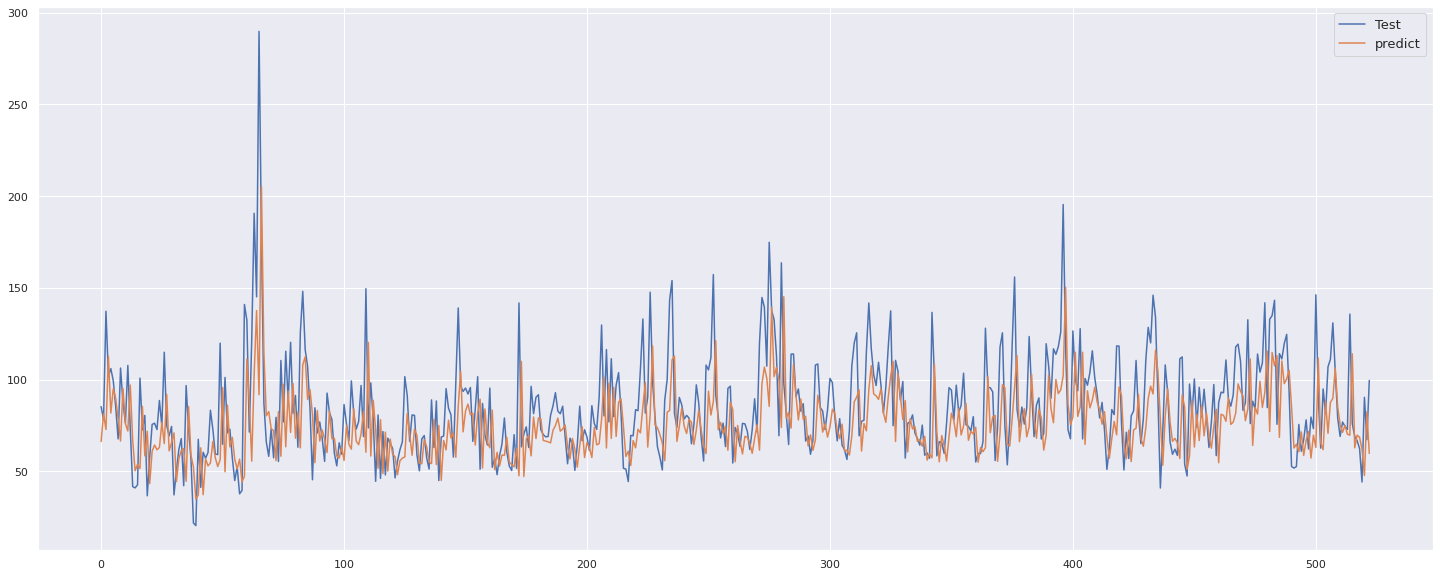
\includegraphics[width=1\linewidth,height=4cm]{model21.png}%
}

\subfloat[Vanilla LSTM model with lambda layer]{
  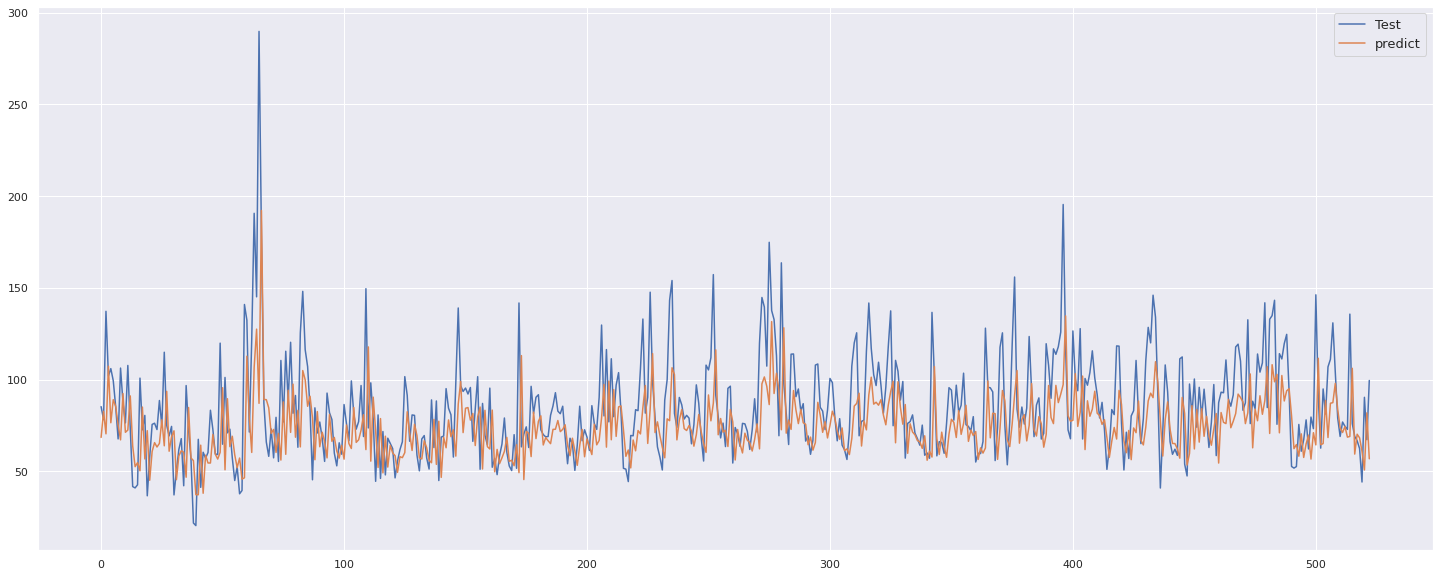
\includegraphics[width=1\linewidth,height=4cm]{model22.png}%
}

\subfloat[Multilayer of LSTM model]{
  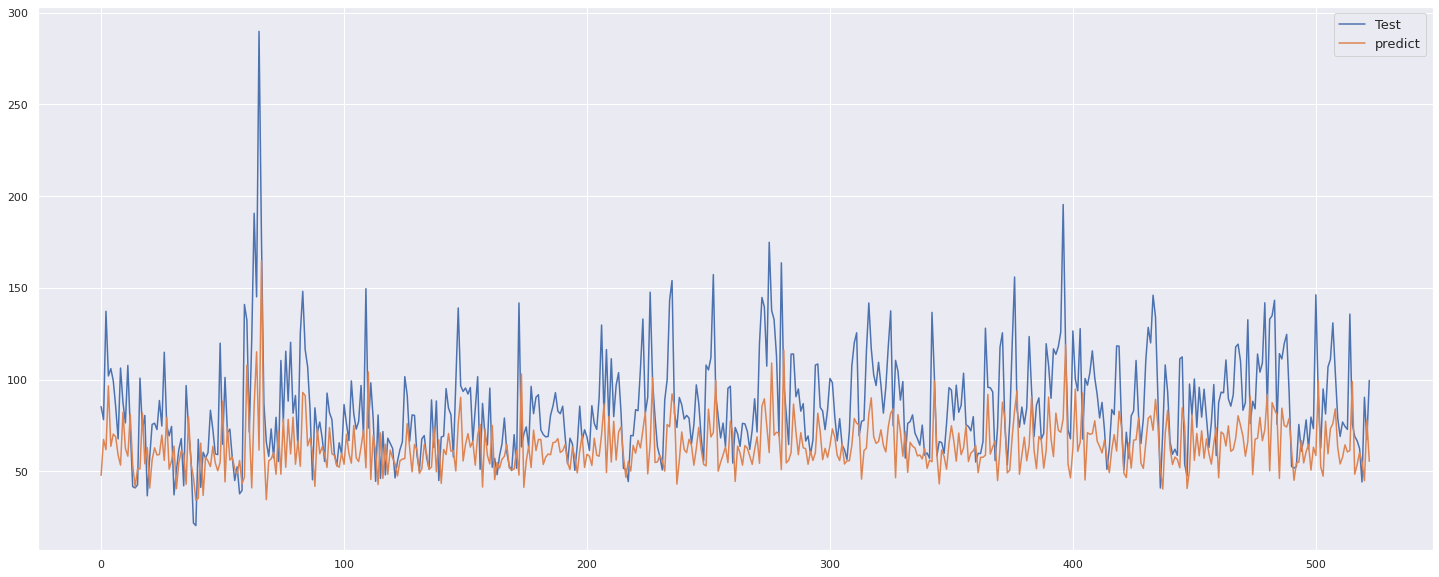
\includegraphics[width=1\linewidth,height=4cm]{model23.png}%
}

\subfloat[single layer Bi-LSTM]{
  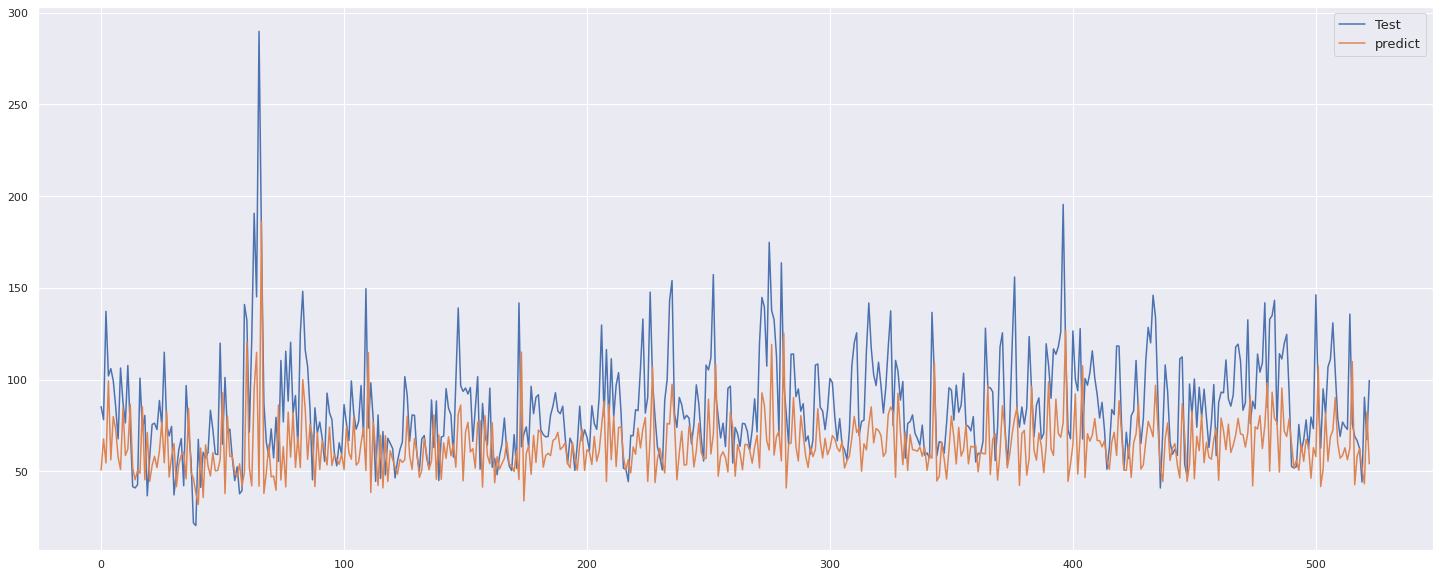
\includegraphics[width=1\linewidth,height=4cm]{model24.png}%
}

\subfloat[multilayer Bi-LSTM model]{
  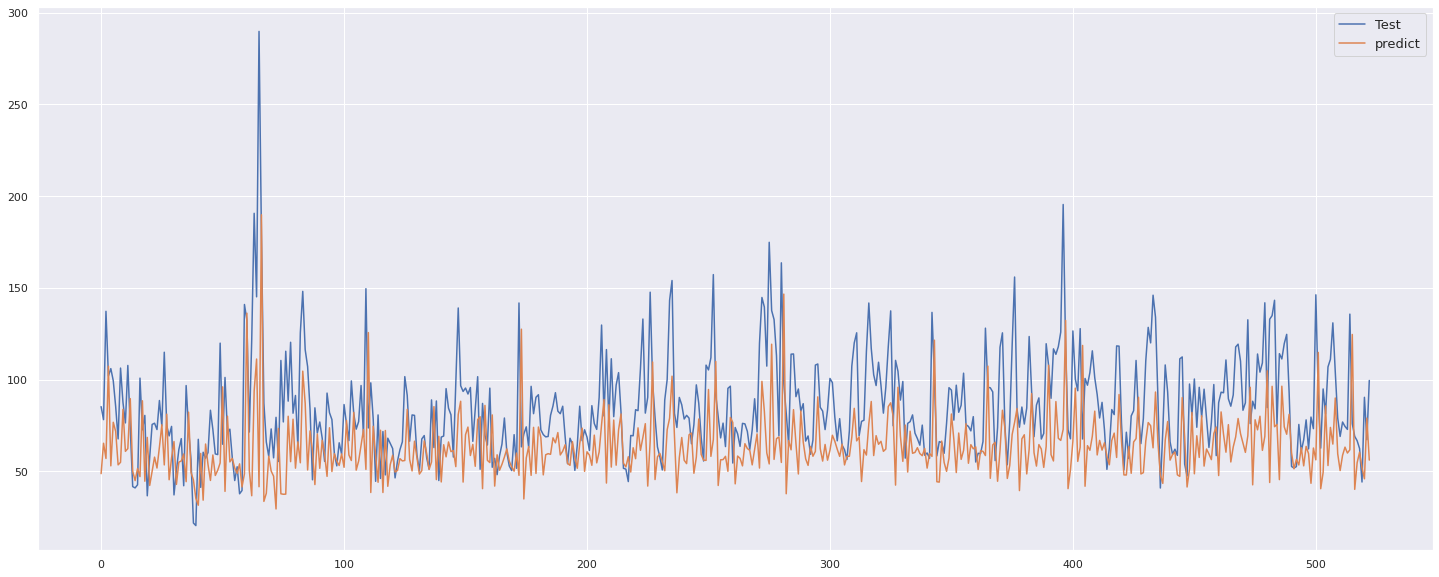
\includegraphics[width=1\linewidth,height=4cm]{model25.png}%
}
\caption{test vs prediction of data on All Model }
\label{fig:vanilla12}
\end{figure}